% This text is proprietary.
% It's a part of presentation made by myself.
% It may not used commercial.
% The noncommercial use such as private and study is free
% Nov. 2006
% Author: Sascha Frank 
% University Freiburg 
% www.informatik.uni-freiburg.de/~frank/
%
% additional usepackage{beamerthemeshadow} is used
%  
%  \beamersetuncovermixins{\opaqueness<1>{25}}{\opaqueness<2->{15}}
%  with this the elements which were coming soon were only hinted
\documentclass{beamer}
\usepackage{beamerthemeshadow}
\usepackage{graphicx}
\usepackage[utf8]{inputenc}  
\usepackage[T1]{fontenc} 
%\usepackage[top=2cm,bottom=2cm,left=2cm,right=2cm,asymmetric]{geometry}

\usepackage{tkz-graph}
\usepackage{amsmath}
\usepackage{array,multirow,makecell}
\usepackage{float}
\usepackage{cancel}
\usepackage{algorithm}
\usepackage{algpseudocode}
\usepackage{subfig}
\usepackage{wrapfig}
\usepackage{ stmaryrd }
\usepackage{placeins}
\usepackage{ amssymb }
\usepackage{mathtools}

\begin{document}
\title{Significant perturbations in observability graph\\}  
\author{Oussama Ennafii \& Sammy Khalife}
\institute{ENS Cachan - Master MVA}
\date{\today} 

\frame{\titlepage} 

%\frame{\frametitle{Table of contents}\tableofcontents} 


\section{Introduction} 


\subsection{Bandit framework}
\frame{ \frametitle{Bandit framework:}
\begin{itemize}
	\item Sequence of losses $(l_t)_{1 \leq t \leq T}$ and actions $(i_t)_{1 \leq t \leq T} $
	~\\
	~\\
	\item Minimax regret $ R(G,T)=\min_{S} \max_{l_1,...,l_T} \mathbb{E}  \sum_{t=1}^{T} l_t(i_t) -\min_{i} \sum_{t=1}^{T}l_t(i)  $
	~\\
\end{itemize}
}

\subsection{Feedback graph:}
\frame{
	\frametitle{Feedback graph}
	
	\begin{itemize}
		\item Directed graph with $K$ nodes corresponding to the possible actions.
		
		\item When a player chooses action $i$ he gets feedback concerning some $j$: this represented by an edge. 
		
		\item A self loop means that whenever the player chooses the action he gets a feedback on it.
	\end{itemize}
	}


\frame{\frametitle{Well-known configuration}
		\begin{figure}
			\centering
			\begin{minipage}{0.45\textwidth}
				\centering
			\caption{Feedback with expert advice}
			\begin{tikzpicture}[
			->,>=stealth',shorten >=1pt,auto,node distance=3cm,
			thick,main node/.style={circle,draw,font=\Large\bfseries}]
			\node[main node] (1) at (0,0) {1};
			\node[main node] (2) at (-1.5,-0.7) {2};
			\node[main node] (3) at (-0.7, -2) {3};
			\node[main node] (4) at (0.7,-2) {4};
			\node[main node] (5) at (1.5,-0.7) {5};
			\path
			(1) edge [loop above] node {} (1);
			\path
			(2) edge [loop below] node {} (2);
			\path
			(3) edge [loop below] node {} (3);
			\path
			(4) edge [loop below] node {} (4);
			\path
			(5) edge [loop below] node {} (5);
			
			\tikzstyle{LabelStyle}=[fill=white,sloped]
			%\tikzstyle{EdgeStyle}=[bend left]
			\Edge[](1)(2)
			\Edge[](1)(3)
			\Edge[](1)(4)
			\Edge[](1)(5)
			\Edge[](2)(4)
			\Edge[](4)(3)
			\Edge[](5)(4)
			\Edge[](5)(3)
			%\tikzstyle{EdgeStyle}=[bend right]
			\Edge[](5)(1)
			\Edge[](4)(1)
			\Edge[](3)(2)
			\Edge[](4)(2)
			\Edge[](3)(4)
			\Edge[](4)(5)
			\Edge[](3)(1)
			\Edge[](3)(5)
			\Edge[](2)(1)
			\end{tikzpicture}
			\end{minipage}\hfill
			\begin{minipage}{0.45\textwidth}
				\centering
				\caption{Bandit feedback}
				\begin{tikzpicture}[->,>=stealth',shorten >=1pt,auto,node distance=3cm,
				thick,main node/.style={circle,draw,font=\Large\bfseries}]
				\node[main node] (1) at (0,0) {1};
				\node[main node] (2) at (-1.5,-0.7) {2};
				\node[main node] (3) at (-0.7, -2) {3};
				\node[main node] (4) at (0.7,-2) {4};
				\node[main node] (5) at (1.5,-0.7) {5};
				\path
				(1) edge [loop above] node {} (1);
				\path
				(2) edge [loop above] node {} (2);
				\path
				(3) edge [loop above] node {} (3);
				\path
				(4) edge [loop above] node {} (4);
				\path
				(5) edge [loop above] node {} (5);
				\end{tikzpicture}
			\end{minipage}
		\end{figure}
}

\subsection{Previous results}

\frame{\frametitle{Previous results}
	Bounds on the minimax regret with respect of the geometry of the graph :
\begin{itemize}
\item Strongly observable with independence number $\alpha$ : $ R(G,T)= \tilde{\Theta}(\alpha^{1/2}T^{1/2})$.
\item Weakly observable with domination number $\delta$ : $ R(G,T) = \tilde{\Theta}(\delta^{1/3}T^{2/3})$
 \item Unobservable : $ R(G,T) = \tilde{\Theta}(T) $.
\end{itemize}
}


\section{Theoretical Study}

\subsection{Definitions:}

\frame{
	\frametitle{Definitions:}
	\begin{block}{Definition:(Observability)}
		Let $G=(V,E)$ be a directed graph. A vertex $v$ is called observable if $N_{in}(v) \neq \emptyset$.\\
		$v$ is strongly observable if it has a self loop or $V\setminus \{v\} \subset N_{in}(v) $. It is weakly observalble in case when it is observable but not strongly.\\
		A graph $G$ is observable if all its vertices are observable and it is strongly observable if all its vertices are strongly observable. A graph is weakly observable if it is observable but not strongly.
		
	\end{block}
	
	}
	
	\frame{
		\frametitle{Definitions:}
		\begin{block}{Definition:(Weak Domination)}
			In a directed graph $ G = (V,E)$ with a set of weakly observable vertices $W \subset V$ , a weakly dominating set $D \subset V$ is a set of vertices that dominates W. Namely, for any $w \in W$ there exists $d \in D$ such that $w \in N_{out}(d)$. The weak domination number of G, denoted by $\delta(G)$, is the size of the smallest weakly dominating set.
			
		\end{block}
		
	}
	
	
	\frame{
		\frametitle{Definitions:}
		\begin{block}{Definition:(Independence)}
			An independent set$ S \subset V$ is a set of vertices that are not connected by any edges. Namely, for any $u,v \in S, u\neq v$ it holds that $(u,v)\notin E$. The independence number $\alpha(G)$ of $G$ is the size of its largest independent set.
			
		\end{block}
		
	}
	
	\subsection{Unstable graphs:}
	
	\frame{
		\frametitle{Stable graphs:}
		If we stay in the same class, adding or deleting one edge would result in:
		\begin{itemize}
			\item The independence number $\alpha$ varies at most by $2$.
			\item The weak domination number $\delta$ varies at most by $1$.
		\end{itemize}
		
		This means that, if the graph stays in the same class, the minimax regret does not change dramatically after perturbing one edge.
		}
		
	\frame{
		\frametitle{Unstable graphs}
		There are three possibilities:
		\begin{itemize}
			\item[(i)] going from strongly observable graphs to weakly observable ones and back.
			\item[(ii)] going from strongly observable graphs to non observable ones and back.
			\item[(iii)] going from weakly observable graphs to non observable ones and back.
		\end{itemize}
		}
	
	\frame{
		\frametitle{Unstable graphs}
		\begin{itemize}
			\item[(i)] In this case, we remove a self loop for an vertice that has other inward edges or we remove an edge for a loop less vertice that also has other inward edges.
			\item[(ii)] When possible, we remove a loop for a vertice that has no other inward edge.
			\item[(iii)] When possible, we remove the only inward edge, that is not a self loop, to such a vertice.
		\end{itemize}
	}
	

\section{Experiments}
\frame{\frametitle{Strongly observable graph}
	\begin{tikzpicture}[->,>=stealth',shorten >=1pt,auto,node distance=3cm,
	thick,main node/.style={circle,draw,font=\Large\bfseries}]
	\node[main node] (1) at (0,0) {1};
	\node[main node] (2) at (-1.5,-1.5) {2};
	\node[main node] (3) at (-0.5, -2) {3};
	\node[main node] (4) at (0.5,-2) {4};
	\node[main node] (5) at (1.5,-1.5) {5};
	\path
	(1) edge [loop above] node {} (1);
	\path
	(2) edge [loop below] node {} (2);
	\path
	(3) edge [loop below] node {} (3);
	\path
	(4) edge [loop below] node {} (4);
	\path
	(5) edge [loop below] node {} (5);
	%edge [bend right] node {0.4} (2)
	%(1) edge node [below]{} (2)
	%%(1) edge [loop below] node {} (3)
	%%edge node[right] {0.1} (1)
	%(1) edge node[below] {} (3); 
	%(1) edge node[below] {} (4);
	%(1) edge node[below] {} (5);    
	\draw (1) -- (2);
	\draw (1) -- (3);
	\draw (1) -- (4);
	\draw (1) -- (5); 
	\end{tikzpicture} 
	\hfill
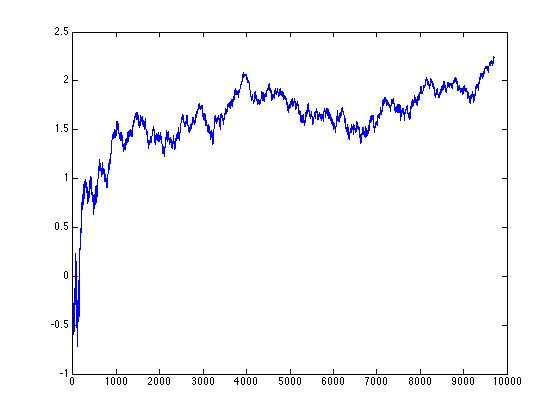
\includegraphics[width=5cm]{logRegretStrongly.jpg}
%\includegraphics[width =0.32\textwidth]{../Code/logRegretWeakly.jpg}
\begin{itemize}
	\item \footnotesize{Revealing action graph, $\alpha=4$}  \qquad \qquad \qquad \footnotesize{Associated log-regret}
	\end{itemize}
}
	
\frame{\frametitle{Weakly observable graph}
		\begin{tikzpicture}[->,>=stealth',shorten >=1pt,auto,node distance=3cm,
		thick,main node/.style={circle,draw,font=\Large\bfseries}]
		
		\node[main node] (1) at (0,0) {1};
		\node[main node] (2) at (-1.5,-1.5) {2};
		\node[main node] (3) at (-0.5, -2) {3};
		\node[main node] (4) at (0.5,-2) {4};
		\node[main node] (5) at (1.5,-1.5) {5};
		\path
		(1) edge [loop above] node {} (1);
		%\path
		%(2) edge [loop below] node {} (2);
		\path
		(3) edge [loop below] node {} (3);
		\path
		(4) edge [loop below] node {} (4);
		\path
		(5) edge [loop below] node {} (5);
		%edge [bend right] node {0.4} (2)
		%(1) edge node [below]{} (2)
		%%(1) edge [loop below] node {} (3)
		%%edge node[right] {0.1} (1)
		%(1) edge node[below] {} (3); 
		%(1) edge node[below] {} (4);
		%(1) edge node[below] {} (5);    
		\draw (1) -- (2);
		\draw (1) -- (3);
		\draw (1) -- (4);
		\draw (1) -- (5);
		\end{tikzpicture}
	\hfill
	\includegraphics[width=5cm]{logRegretWeakly.jpg}
	\begin{itemize}
	\item \footnotesize{Pertubed graph, $\delta = 1$} \qquad \qquad  \qquad \qquad \footnotesize{Associated log-regret }
	\end{itemize}
}

\frame{\frametitle{Non observable graph}
\begin{tikzpicture}[->,>=stealth',shorten >=1pt,auto,node distance=3cm,
thick,main node/.style={circle,draw,font=\Large\bfseries}]

\node[main node] (1) at (0,0) {1};
\node[main node] (2) at (-1.5,-1.5) {2};
\node[main node] (3) at (-0.5, -2) {3};
\node[main node] (4) at (0.5,-2) {4};
\node[main node] (5) at (1.5,-1.5) {5};
%\path
%(1) edge [loop above] node {} (1);
\path
(2) edge [loop below] node {} (2);
\path
(3) edge [loop below] node {} (3);
\path
(4) edge [loop below] node {} (4);
\path
(5) edge [loop below] node {} (5);
%edge [bend right] node {0.4} (2)
%(1) edge node [below]{} (2)
%%(1) edge [loop below] node {} (3)
%%edge node[right] {0.1} (1)
%(1) edge node[below] {} (3); 
%(1) edge node[below] {} (4);
%(1) edge node[below] {} (5);    
\draw (1) -- (2);
\draw (1) -- (3);
\draw (1) -- (4);
\draw (1) -- (5);
\end{tikzpicture} 
			\hfill
			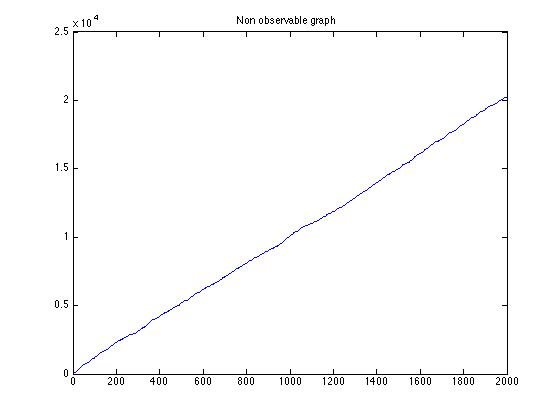
\includegraphics[width=5cm]{regretNonObservable.jpg}
			\begin{itemize}
				\item \footnotesize{Node 1 non observable} \qquad \qquad  \qquad \qquad \footnotesize{Associated log-regret }
			\end{itemize}
	}
\end{document}






